\documentclass[1p]{elsarticle_modified}
%\bibliographystyle{elsarticle-num}

%\usepackage[colorlinks]{hyperref}
%\usepackage{abbrmath_seonhwa} %\Abb, \Ascr, \Acal ,\Abf, \Afrak
\usepackage{amsfonts}
\usepackage{amssymb}
\usepackage{amsmath}
\usepackage{amsthm}
\usepackage{scalefnt}
\usepackage{amsbsy}
\usepackage{kotex}
\usepackage{caption}
\usepackage{subfig}
\usepackage{color}
\usepackage{graphicx}
\usepackage{xcolor} %% white, black, red, green, blue, cyan, magenta, yellow
\usepackage{float}
\usepackage{setspace}
\usepackage{hyperref}

\usepackage{tikz}
\usetikzlibrary{arrows}

\usepackage{multirow}
\usepackage{array} % fixed length table
\usepackage{hhline}

%%%%%%%%%%%%%%%%%%%%%
\makeatletter
\renewcommand*\env@matrix[1][\arraystretch]{%
	\edef\arraystretch{#1}%
	\hskip -\arraycolsep
	\let\@ifnextchar\new@ifnextchar
	\array{*\c@MaxMatrixCols c}}
\makeatother %https://tex.stackexchange.com/questions/14071/how-can-i-increase-the-line-spacing-in-a-matrix
%%%%%%%%%%%%%%%

\usepackage[normalem]{ulem}

\newcommand{\msout}[1]{\ifmmode\text{\sout{\ensuremath{#1}}}\else\sout{#1}\fi}
%SOURCE: \msout is \stkout macro in https://tex.stackexchange.com/questions/20609/strikeout-in-math-mode

\newcommand{\cancel}[1]{
	\ifmmode
	{\color{red}\msout{#1}}
	\else
	{\color{red}\sout{#1}}
	\fi
}

\newcommand{\add}[1]{
	{\color{blue}\uwave{#1}}
}

\newcommand{\replace}[2]{
	\ifmmode
	{\color{red}\msout{#1}}{\color{blue}\uwave{#2}}
	\else
	{\color{red}\sout{#1}}{\color{blue}\uwave{#2}}
	\fi
}

\newcommand{\Sol}{\mathcal{S}} %segment
\newcommand{\D}{D} %diagram
\newcommand{\A}{\mathcal{A}} %arc


%%%%%%%%%%%%%%%%%%%%%%%%%%%%%5 test

\def\sl{\operatorname{\textup{SL}}(2,\Cbb)}
\def\psl{\operatorname{\textup{PSL}}(2,\Cbb)}
\def\quan{\mkern 1mu \triangleright \mkern 1mu}

\theoremstyle{definition}
\newtheorem{thm}{Theorem}[section]
\newtheorem{prop}[thm]{Proposition}
\newtheorem{lem}[thm]{Lemma}
\newtheorem{ques}[thm]{Question}
\newtheorem{cor}[thm]{Corollary}
\newtheorem{defn}[thm]{Definition}
\newtheorem{exam}[thm]{Example}
\newtheorem{rmk}[thm]{Remark}
\newtheorem{alg}[thm]{Algorithm}

\newcommand{\I}{\sqrt{-1}}
\begin{document}

%\begin{frontmatter}
%
%\title{Boundary parabolic representations of knots up to 8 crossings}
%
%%% Group authors per affiliation:
%\author{Yunhi Cho} 
%\address{Department of Mathematics, University of Seoul, Seoul, Korea}
%\ead{yhcho@uos.ac.kr}
%
%
%\author{Seonhwa Kim} %\fnref{s_kim}}
%\address{Center for Geometry and Physics, Institute for Basic Science, Pohang, 37673, Korea}
%\ead{ryeona17@ibs.re.kr}
%
%\author{Hyuk Kim}
%\address{Department of Mathematical Sciences, Seoul National University, Seoul 08826, Korea}
%\ead{hyukkim@snu.ac.kr}
%
%\author{Seokbeom Yoon}
%\address{Department of Mathematical Sciences, Seoul National University, Seoul, 08826,  Korea}
%\ead{sbyoon15@snu.ac.kr}
%
%\begin{abstract}
%We find all boundary parabolic representation of knots up to 8 crossings.
%
%\end{abstract}
%\begin{keyword}
%    \MSC[2010] 57M25 
%\end{keyword}
%
%\end{frontmatter}

%\linenumbers
%\tableofcontents
%
\newcommand\colored[1]{\textcolor{white}{\rule[-0.35ex]{0.8em}{1.4ex}}\kern-0.8em\color{red} #1}%
%\newcommand\colored[1]{\textcolor{white}{ #1}\kern-2.17ex	\textcolor{white}{ #1}\kern-1.81ex	\textcolor{white}{ #1}\kern-2.15ex\color{red}#1	}

{\Large $\underline{12n_{0192}~(K12n_{0192})}$}

\setlength{\tabcolsep}{10pt}
\renewcommand{\arraystretch}{1.6}
\vspace{1cm}\begin{tabular}{m{100pt}>{\centering\arraybackslash}m{274pt}}
\multirow{5}{120pt}{
	\centering
	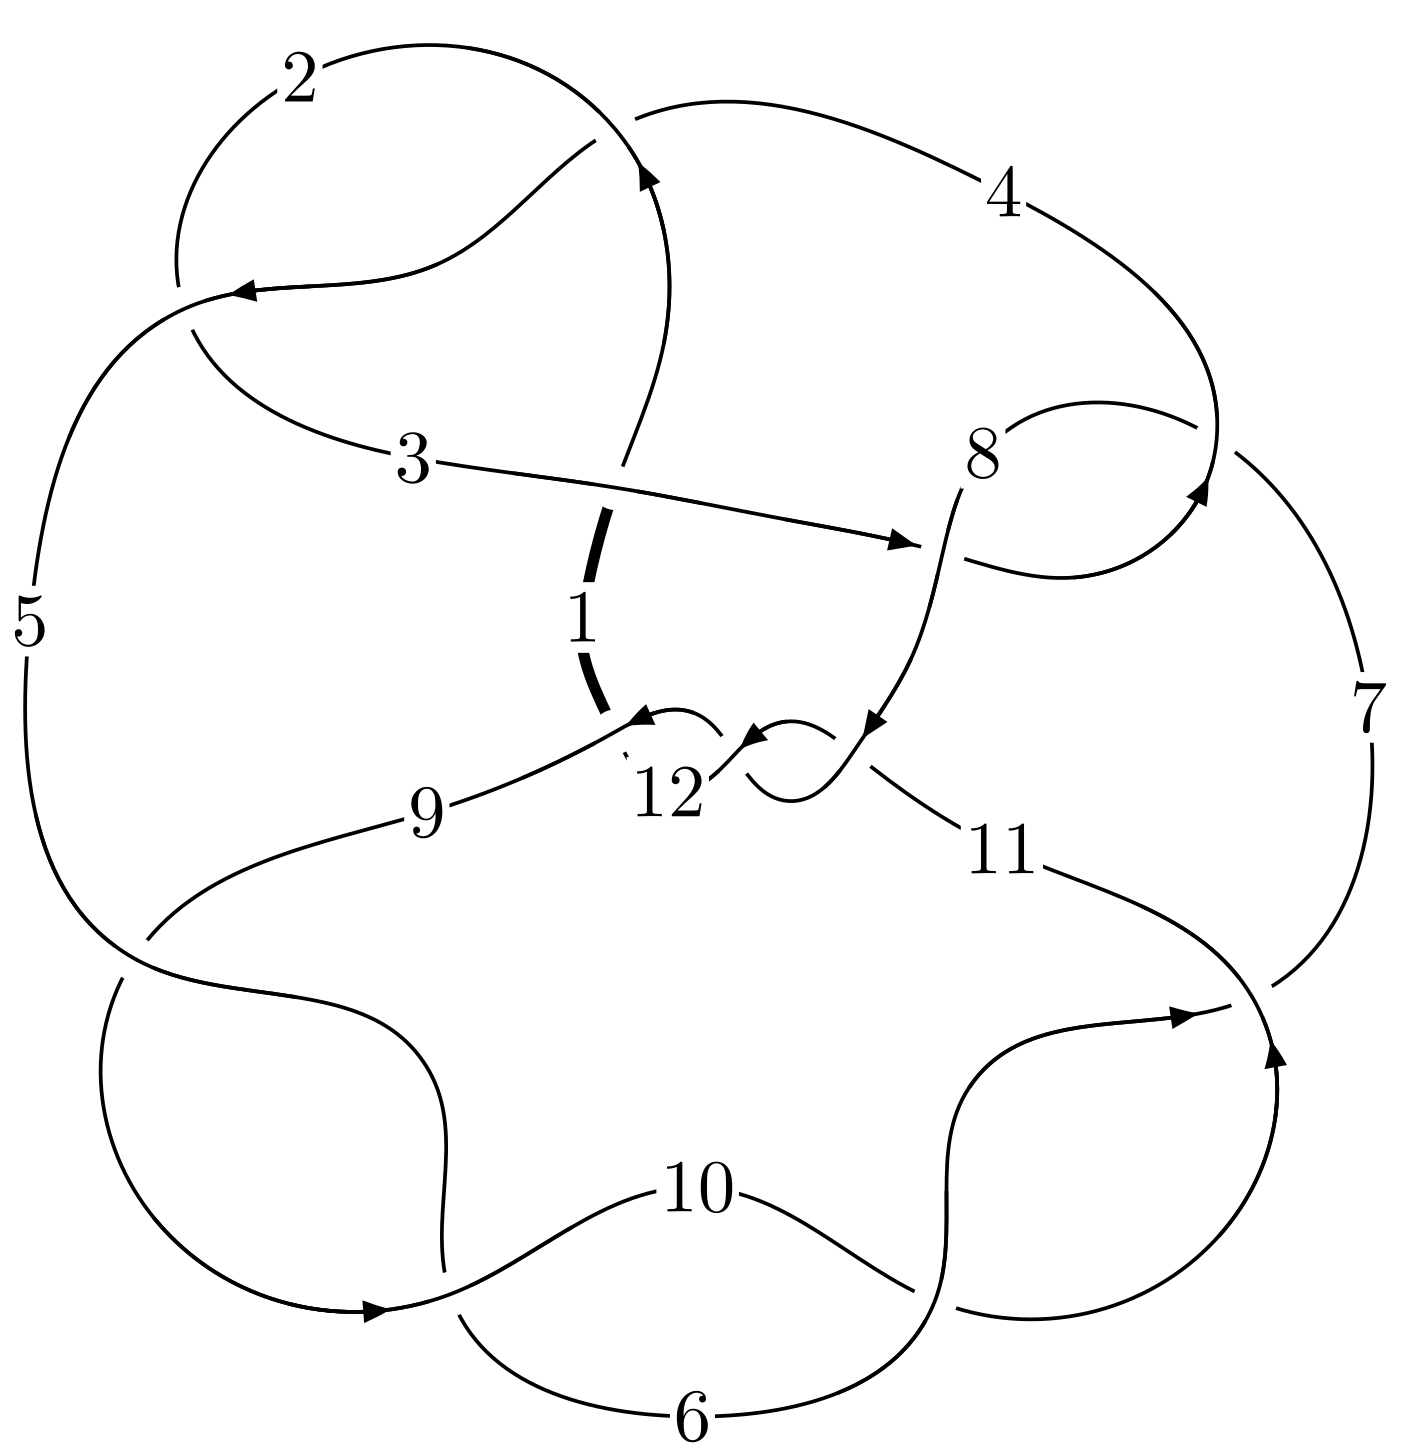
\includegraphics[width=112pt]{../../../GIT/diagram.site/Diagrams/png/2281_12n_0192.png}\\
\ \ \ A knot diagram\footnotemark}&
\allowdisplaybreaks
\textbf{Linearized knot diagam} \\
\cline{2-2}
 &
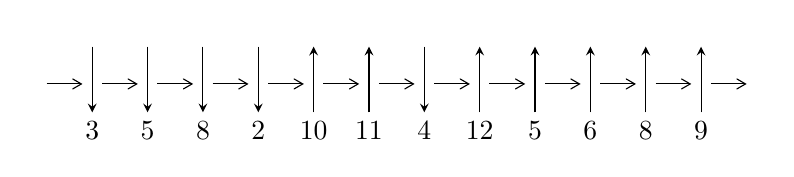
\begin{tikzpicture}[x=20pt, y=17pt]
	% nodes
	\node (C0) at (0, 0) {};
	\node (C1) at (1, 0) {};
	\node (C1U) at (1, +1) {};
	\node (C1D) at (1, -1) {3};

	\node (C2) at (2, 0) {};
	\node (C2U) at (2, +1) {};
	\node (C2D) at (2, -1) {5};

	\node (C3) at (3, 0) {};
	\node (C3U) at (3, +1) {};
	\node (C3D) at (3, -1) {8};

	\node (C4) at (4, 0) {};
	\node (C4U) at (4, +1) {};
	\node (C4D) at (4, -1) {2};

	\node (C5) at (5, 0) {};
	\node (C5U) at (5, +1) {};
	\node (C5D) at (5, -1) {10};

	\node (C6) at (6, 0) {};
	\node (C6U) at (6, +1) {};
	\node (C6D) at (6, -1) {11};

	\node (C7) at (7, 0) {};
	\node (C7U) at (7, +1) {};
	\node (C7D) at (7, -1) {4};

	\node (C8) at (8, 0) {};
	\node (C8U) at (8, +1) {};
	\node (C8D) at (8, -1) {12};

	\node (C9) at (9, 0) {};
	\node (C9U) at (9, +1) {};
	\node (C9D) at (9, -1) {5};

	\node (C10) at (10, 0) {};
	\node (C10U) at (10, +1) {};
	\node (C10D) at (10, -1) {6};

	\node (C11) at (11, 0) {};
	\node (C11U) at (11, +1) {};
	\node (C11D) at (11, -1) {8};

	\node (C12) at (12, 0) {};
	\node (C12U) at (12, +1) {};
	\node (C12D) at (12, -1) {9};
	\node (C13) at (13, 0) {};

	% arrows
	\draw[->,>={angle 60}]
	(C0) edge (C1) (C1) edge (C2) (C2) edge (C3) (C3) edge (C4) (C4) edge (C5) (C5) edge (C6) (C6) edge (C7) (C7) edge (C8) (C8) edge (C9) (C9) edge (C10) (C10) edge (C11) (C11) edge (C12) (C12) edge (C13) ;	\draw[->,>=stealth]
	(C1U) edge (C1D) (C2U) edge (C2D) (C3U) edge (C3D) (C4U) edge (C4D) (C5D) edge (C5U) (C6D) edge (C6U) (C7U) edge (C7D) (C8D) edge (C8U) (C9D) edge (C9U) (C10D) edge (C10U) (C11D) edge (C11U) (C12D) edge (C12U) ;
	\end{tikzpicture} \\
\hhline{~~} \\& 
\textbf{Solving Sequence} \\ \cline{2-2} 
 &
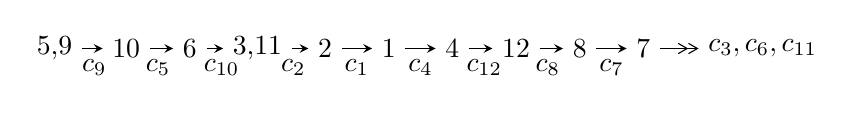
\begin{tikzpicture}[x=23pt, y=7pt]
	% node
	\node (A0) at (-1/8, 0) {5,9};
	\node (A1) at (1, 0) {10};
	\node (A2) at (2, 0) {6};
	\node (A3) at (49/16, 0) {3,11};
	\node (A4) at (33/8, 0) {2};
	\node (A5) at (41/8, 0) {1};
	\node (A6) at (49/8, 0) {4};
	\node (A7) at (57/8, 0) {12};
	\node (A8) at (65/8, 0) {8};
	\node (A9) at (73/8, 0) {7};
	\node (C1) at (1/2, -1) {$c_{9}$};
	\node (C2) at (3/2, -1) {$c_{5}$};
	\node (C3) at (5/2, -1) {$c_{10}$};
	\node (C4) at (29/8, -1) {$c_{2}$};
	\node (C5) at (37/8, -1) {$c_{1}$};
	\node (C6) at (45/8, -1) {$c_{4}$};
	\node (C7) at (53/8, -1) {$c_{12}$};
	\node (C8) at (61/8, -1) {$c_{8}$};
	\node (C9) at (69/8, -1) {$c_{7}$};
	\node (A10) at (11, 0) {$c_{3},c_{6},c_{11}$};

	% edge
	\draw[->,>=stealth]	
	(A0) edge (A1) (A1) edge (A2) (A2) edge (A3) (A3) edge (A4) (A4) edge (A5) (A5) edge (A6) (A6) edge (A7) (A7) edge (A8) (A8) edge (A9) ;
	\draw[->>,>={angle 60}]	
	(A9) edge (A10);
\end{tikzpicture} \\ 

\end{tabular} \\

\footnotetext{
The image of knot diagram is generated by the software ``\textbf{Draw programme}" developed by Andrew Bartholomew(\url{http://www.layer8.co.uk/maths/draw/index.htm\#Running-draw}), where we modified some parts for our purpose(\url{https://github.com/CATsTAILs/LinksPainter}).
}\phantom \\ \newline 
\centering \textbf{Ideals for irreducible components\footnotemark of $X_{\text{par}}$} 
 
\begin{align*}
I^u_{1}&=\langle 
-3.17034\times10^{19} u^{22}+2.06027\times10^{19} u^{21}+\cdots+1.07970\times10^{20} b+1.66107\times10^{20},\\
\phantom{I^u_{1}}&\phantom{= \langle  }-9.79843\times10^{18} u^{22}-2.69589\times10^{19} u^{21}+\cdots+2.15940\times10^{20} a-7.11427\times10^{20},\\
\phantom{I^u_{1}}&\phantom{= \langle  }u^{23}-2 u^{22}+\cdots-24 u+8\rangle \\
I^u_{2}&=\langle 
-2 a^2- a u+b-2 a- u-1,\;4 a^3+2 a^2 u- u,\;u^2-2\rangle \\
I^u_{3}&=\langle 
b+u-1,\;u^2+a- u-2,\;u^3- u^2-2 u+1\rangle \\
\\
I^v_{1}&=\langle 
a,\;b+v+2,\;v^3+3 v^2+2 v-1\rangle \\
\end{align*}
\raggedright * 4 irreducible components of $\dim_{\mathbb{C}}=0$, with total 35 representations.\\
\footnotetext{All coefficients of polynomials are rational numbers. But the coefficients are sometimes approximated in decimal forms when there is not enough margin.}
\newpage
\renewcommand{\arraystretch}{1}
\centering \section*{I. $I^u_{1}= \langle -3.17\times10^{19} u^{22}+2.06\times10^{19} u^{21}+\cdots+1.08\times10^{20} b+1.66\times10^{20},\;-9.80\times10^{18} u^{22}-2.70\times10^{19} u^{21}+\cdots+2.16\times10^{20} a-7.11\times10^{20},\;u^{23}-2 u^{22}+\cdots-24 u+8 \rangle$}
\flushleft \textbf{(i) Arc colorings}\\
\begin{tabular}{m{7pt} m{180pt} m{7pt} m{180pt} }
\flushright $a_{5}=$&$\begin{pmatrix}0\\u\end{pmatrix}$ \\
\flushright $a_{9}=$&$\begin{pmatrix}1\\0\end{pmatrix}$ \\
\flushright $a_{10}=$&$\begin{pmatrix}1\\- u^2\end{pmatrix}$ \\
\flushright $a_{6}=$&$\begin{pmatrix}u\\- u^3+u\end{pmatrix}$ \\
\flushright $a_{3}=$&$\begin{pmatrix}0.0453756 u^{22}+0.124844 u^{21}+\cdots+6.96611 u+3.29455\\0.293631 u^{22}-0.190818 u^{21}+\cdots+6.03607 u-1.53845\end{pmatrix}$ \\
\flushright $a_{11}=$&$\begin{pmatrix}- u^2+1\\u^4-2 u^2\end{pmatrix}$ \\
\flushright $a_{2}=$&$\begin{pmatrix}0.0453756 u^{22}+0.124844 u^{21}+\cdots+6.96611 u+3.29455\\-0.0606713 u^{22}+0.0493494 u^{21}+\cdots+1.22479 u+0.186315\end{pmatrix}$ \\
\flushright $a_{1}=$&$\begin{pmatrix}0.00815407 u^{22}+0.0581561 u^{21}+\cdots+0.816899 u+0.942300\\0.167916 u^{22}-0.134620 u^{21}+\cdots+3.19264 u-1.46520\end{pmatrix}$ \\
\flushright $a_{4}=$&$\begin{pmatrix}-0.318134 u^{22}+0.323483 u^{21}+\cdots+1.70680 u+4.47989\\0.354835 u^{22}-0.251401 u^{21}+\cdots+7.02928 u-1.98143\end{pmatrix}$ \\
\flushright $a_{12}=$&$\begin{pmatrix}-0.159762 u^{22}+0.192776 u^{21}+\cdots-2.37574 u+2.40750\\0.167916 u^{22}-0.134620 u^{21}+\cdots+3.19264 u-1.46520\end{pmatrix}$ \\
\flushright $a_{8}=$&$\begin{pmatrix}-0.231610 u^{22}+0.238881 u^{21}+\cdots-3.80455 u+2.85872\\0.190322 u^{22}-0.136611 u^{21}+\cdots+2.10246 u-1.34349\end{pmatrix}$ \\
\flushright $a_{7}=$&$\begin{pmatrix}u^3-2 u\\- u^5+3 u^3- u\end{pmatrix}$\\&\end{tabular}
\flushleft \textbf{(ii) Obstruction class $= -1$}\\~\\
\flushleft \textbf{(iii) Cusp Shapes $= \frac{158891265015344169787}{107970245740225855892} u^{22}-\frac{49683941378257544770}{26992561435056463973} u^{21}+\cdots-\frac{765639597674599940106}{26992561435056463973} u-\frac{395673949272391412502}{26992561435056463973}$}\\~\\
\newpage\renewcommand{\arraystretch}{1}
\flushleft \textbf{(iv) u-Polynomials at the component}\newline \\
\begin{tabular}{m{50pt}|m{274pt}}
Crossings & \hspace{64pt}u-Polynomials at each crossing \\
\hline $$\begin{aligned}c_{1}\end{aligned}$$&$\begin{aligned}
&u^{23}+23 u^{22}+\cdots+431 u+1
\end{aligned}$\\
\hline $$\begin{aligned}c_{2},c_{4}\end{aligned}$$&$\begin{aligned}
&u^{23}-7 u^{22}+\cdots-25 u-1
\end{aligned}$\\
\hline $$\begin{aligned}c_{3},c_{7}\end{aligned}$$&$\begin{aligned}
&u^{23}+2 u^{22}+\cdots-92 u+8
\end{aligned}$\\
\hline $$\begin{aligned}c_{5},c_{6},c_{9}\\c_{10}\end{aligned}$$&$\begin{aligned}
&u^{23}+2 u^{22}+\cdots-24 u-8
\end{aligned}$\\
\hline $$\begin{aligned}c_{8},c_{11},c_{12}\end{aligned}$$&$\begin{aligned}
&u^{23}-5 u^{22}+\cdots+105 u-7
\end{aligned}$\\
\hline
\end{tabular}\\~\\
\newpage\renewcommand{\arraystretch}{1}
\flushleft \textbf{(v) Riley Polynomials at the component}\newline \\
\begin{tabular}{m{50pt}|m{274pt}}
Crossings & \hspace{64pt}Riley Polynomials at each crossing \\
\hline $$\begin{aligned}c_{1}\end{aligned}$$&$\begin{aligned}
&y^{23}-39 y^{22}+\cdots+167215 y-1
\end{aligned}$\\
\hline $$\begin{aligned}c_{2},c_{4}\end{aligned}$$&$\begin{aligned}
&y^{23}-23 y^{22}+\cdots+431 y-1
\end{aligned}$\\
\hline $$\begin{aligned}c_{3},c_{7}\end{aligned}$$&$\begin{aligned}
&y^{23}-12 y^{22}+\cdots+4048 y-64
\end{aligned}$\\
\hline $$\begin{aligned}c_{5},c_{6},c_{9}\\c_{10}\end{aligned}$$&$\begin{aligned}
&y^{23}-18 y^{22}+\cdots+1984 y-64
\end{aligned}$\\
\hline $$\begin{aligned}c_{8},c_{11},c_{12}\end{aligned}$$&$\begin{aligned}
&y^{23}-3 y^{22}+\cdots+3857 y-49
\end{aligned}$\\
\hline
\end{tabular}\\~\\
\newpage\flushleft \textbf{(vi) Complex Volumes and Cusp Shapes}
$$\begin{array}{c|c|c}  
\text{Solutions to }I^u_{1}& \I (\text{vol} + \sqrt{-1}CS) & \text{Cusp shape}\\
 \hline 
\begin{aligned}
u &= \phantom{-}0.524450 + 0.823406 I \\
a &= \phantom{-}1.198540 - 0.301680 I \\
b &= -0.0820455 - 0.0681602 I\end{aligned}
 & -2.40419 - 0.36830 I & \phantom{-}2.14910 - 0.07440 I \\ \hline\begin{aligned}
u &= \phantom{-}0.524450 - 0.823406 I \\
a &= \phantom{-}1.198540 + 0.301680 I \\
b &= -0.0820455 + 0.0681602 I\end{aligned}
 & -2.40419 + 0.36830 I & \phantom{-}2.14910 + 0.07440 I \\ \hline\begin{aligned}
u &= \phantom{-}0.647880 + 0.361661 I \\
a &= -1.60944 - 0.06303 I \\
b &= \phantom{-}0.610235 + 0.499402 I\end{aligned}
 & \phantom{-}5.21554 - 2.25150 I & \phantom{-}8.85155 - 0.03890 I \\ \hline\begin{aligned}
u &= \phantom{-}0.647880 - 0.361661 I \\
a &= -1.60944 + 0.06303 I \\
b &= \phantom{-}0.610235 - 0.499402 I\end{aligned}
 & \phantom{-}5.21554 + 2.25150 I & \phantom{-}8.85155 + 0.03890 I \\ \hline\begin{aligned}
u &= -0.968334 + 0.805177 I \\
a &= -0.791369 - 0.993332 I \\
b &= \phantom{-}0.30258 - 1.86935 I\end{aligned}
 & -3.71088 - 3.05913 I & \phantom{-}3.40896 + 2.62935 I \\ \hline\begin{aligned}
u &= -0.968334 - 0.805177 I \\
a &= -0.791369 + 0.993332 I \\
b &= \phantom{-}0.30258 + 1.86935 I\end{aligned}
 & -3.71088 + 3.05913 I & \phantom{-}3.40896 - 2.62935 I \\ \hline\begin{aligned}
u &= \phantom{-}1.348180 + 0.047266 I \\
a &= -0.707662 - 0.573551 I \\
b &= \phantom{-}0.028918 - 1.035860 I\end{aligned}
 & \phantom{-}7.94226 - 2.99119 I & \phantom{-}5.45880 + 3.25887 I \\ \hline\begin{aligned}
u &= \phantom{-}1.348180 - 0.047266 I \\
a &= -0.707662 + 0.573551 I \\
b &= \phantom{-}0.028918 + 1.035860 I\end{aligned}
 & \phantom{-}7.94226 + 2.99119 I & \phantom{-}5.45880 - 3.25887 I \\ \hline\begin{aligned}
u &= \phantom{-}1.37411\phantom{ +0.000000I} \\
a &= \phantom{-}0.0360037\phantom{ +0.000000I} \\
b &= \phantom{-}1.16320\phantom{ +0.000000I}\end{aligned}
 & \phantom{-}6.50526\phantom{ +0.000000I} & \phantom{-}14.0870\phantom{ +0.000000I} \\ \hline\begin{aligned}
u &= -0.596550 + 0.120314 I \\
a &= -0.457301 - 0.724116 I \\
b &= -0.799393 - 0.727747 I\end{aligned}
 & \phantom{-}0.931592 - 0.038203 I & \phantom{-}9.32722 + 1.98466 I\\
 \hline 
 \end{array}$$\newpage$$\begin{array}{c|c|c}  
\text{Solutions to }I^u_{1}& \I (\text{vol} + \sqrt{-1}CS) & \text{Cusp shape}\\
 \hline 
\begin{aligned}
u &= -0.596550 - 0.120314 I \\
a &= -0.457301 + 0.724116 I \\
b &= -0.799393 + 0.727747 I\end{aligned}
 & \phantom{-}0.931592 + 0.038203 I & \phantom{-}9.32722 - 1.98466 I \\ \hline\begin{aligned}
u &= \phantom{-}1.253460 + 0.611260 I \\
a &= -0.257061 - 0.819047 I \\
b &= -0.178277 - 0.996927 I\end{aligned}
 & -0.01572 + 5.94333 I & \phantom{-}6.39784 - 4.46809 I \\ \hline\begin{aligned}
u &= \phantom{-}1.253460 - 0.611260 I \\
a &= -0.257061 + 0.819047 I \\
b &= -0.178277 + 0.996927 I\end{aligned}
 & -0.01572 - 5.94333 I & \phantom{-}6.39784 + 4.46809 I \\ \hline\begin{aligned}
u &= -1.42929\phantom{ +0.000000I} \\
a &= -0.686494\phantom{ +0.000000I} \\
b &= -12.0652\phantom{ +0.000000I}\end{aligned}
 & \phantom{-}4.96770\phantom{ +0.000000I} & -112.550\phantom{ +0.000000I} \\ \hline\begin{aligned}
u &= -0.25726 + 1.43341 I \\
a &= -0.014716 + 1.238780 I \\
b &= -0.02116 + 1.93499 I\end{aligned}
 & -11.10700 - 5.35109 I & \phantom{-}2.30683 + 2.56727 I \\ \hline\begin{aligned}
u &= -0.25726 - 1.43341 I \\
a &= -0.014716 - 1.238780 I \\
b &= -0.02116 - 1.93499 I\end{aligned}
 & -11.10700 + 5.35109 I & \phantom{-}2.30683 - 2.56727 I \\ \hline\begin{aligned}
u &= -0.444315\phantom{ +0.000000I} \\
a &= -0.534871\phantom{ +0.000000I} \\
b &= -0.856360\phantom{ +0.000000I}\end{aligned}
 & \phantom{-}0.878779\phantom{ +0.000000I} & \phantom{-}12.7060\phantom{ +0.000000I} \\ \hline\begin{aligned}
u &= \phantom{-}1.59666 + 0.55985 I \\
a &= -0.723361 + 0.626398 I \\
b &= \phantom{-}0.55500 + 2.06165 I\end{aligned}
 & -5.20585 + 12.38690 I & \phantom{-}5.26515 - 5.63238 I \\ \hline\begin{aligned}
u &= \phantom{-}1.59666 - 0.55985 I \\
a &= -0.723361 - 0.626398 I \\
b &= \phantom{-}0.55500 - 2.06165 I\end{aligned}
 & -5.20585 - 12.38690 I & \phantom{-}5.26515 + 5.63238 I \\ \hline\begin{aligned}
u &= -1.49695 + 0.90558 I \\
a &= \phantom{-}0.809749 + 0.607559 I \\
b &= -0.42702 + 1.59069 I\end{aligned}
 & -7.48548 - 2.83924 I & \phantom{-}3.01997 + 1.35778 I\\
 \hline 
 \end{array}$$\newpage$$\begin{array}{c|c|c}  
\text{Solutions to }I^u_{1}& \I (\text{vol} + \sqrt{-1}CS) & \text{Cusp shape}\\
 \hline 
\begin{aligned}
u &= -1.49695 - 0.90558 I \\
a &= \phantom{-}0.809749 - 0.607559 I \\
b &= -0.42702 - 1.59069 I\end{aligned}
 & -7.48548 + 2.83924 I & \phantom{-}3.01997 - 1.35778 I \\ \hline\begin{aligned}
u &= \phantom{-}0.244699\phantom{ +0.000000I} \\
a &= \phantom{-}3.66585\phantom{ +0.000000I} \\
b &= \phantom{-}0.520617\phantom{ +0.000000I}\end{aligned}
 & -1.28182\phantom{ +0.000000I} & -11.3970\phantom{ +0.000000I} \\ \hline\begin{aligned}
u &= -1.84826\phantom{ +0.000000I} \\
a &= \phantom{-}0.624762\phantom{ +0.000000I} \\
b &= -0.739954\phantom{ +0.000000I}\end{aligned}
 & \phantom{-}15.6748\phantom{ +0.000000I} & -4.21640\phantom{ +0.000000I}\\
 \hline 
 \end{array}$$\newpage\newpage\renewcommand{\arraystretch}{1}
\centering \section*{II. $I^u_{2}= \langle -2 a^2- a u+b-2 a- u-1,\;4 a^3+2 a^2 u- u,\;u^2-2 \rangle$}
\flushleft \textbf{(i) Arc colorings}\\
\begin{tabular}{m{7pt} m{180pt} m{7pt} m{180pt} }
\flushright $a_{5}=$&$\begin{pmatrix}0\\u\end{pmatrix}$ \\
\flushright $a_{9}=$&$\begin{pmatrix}1\\0\end{pmatrix}$ \\
\flushright $a_{10}=$&$\begin{pmatrix}1\\-2\end{pmatrix}$ \\
\flushright $a_{6}=$&$\begin{pmatrix}u\\- u\end{pmatrix}$ \\
\flushright $a_{3}=$&$\begin{pmatrix}a\\2 a^2+a u+2 a+u+1\end{pmatrix}$ \\
\flushright $a_{11}=$&$\begin{pmatrix}-1\\0\end{pmatrix}$ \\
\flushright $a_{2}=$&$\begin{pmatrix}a\\2 a^2+a u+u+1\end{pmatrix}$ \\
\flushright $a_{1}=$&$\begin{pmatrix}a^2 u+a-\frac{1}{2} u\\1\end{pmatrix}$ \\
\flushright $a_{4}=$&$\begin{pmatrix}a^2 u\\a u+2 a+u+1\end{pmatrix}$ \\
\flushright $a_{12}=$&$\begin{pmatrix}a^2 u+a-\frac{1}{2} u-1\\1\end{pmatrix}$ \\
\flushright $a_{8}=$&$\begin{pmatrix}a^2 u+a-\frac{1}{2} u\\1\end{pmatrix}$ \\
\flushright $a_{7}=$&$\begin{pmatrix}0\\- u\end{pmatrix}$\\&\end{tabular}
\flushleft \textbf{(ii) Obstruction class $= 1$}\\~\\
\flushleft \textbf{(iii) Cusp Shapes $= -4 a u+8$}\\~\\
\newpage\renewcommand{\arraystretch}{1}
\flushleft \textbf{(iv) u-Polynomials at the component}\newline \\
\begin{tabular}{m{50pt}|m{274pt}}
Crossings & \hspace{64pt}u-Polynomials at each crossing \\
\hline $$\begin{aligned}c_{1},c_{7}\end{aligned}$$&$\begin{aligned}
&(u^3- u^2+2 u-1)^2
\end{aligned}$\\
\hline $$\begin{aligned}c_{2}\end{aligned}$$&$\begin{aligned}
&(u^3+u^2-1)^2
\end{aligned}$\\
\hline $$\begin{aligned}c_{3}\end{aligned}$$&$\begin{aligned}
&(u^3+u^2+2 u+1)^2
\end{aligned}$\\
\hline $$\begin{aligned}c_{4}\end{aligned}$$&$\begin{aligned}
&(u^3- u^2+1)^2
\end{aligned}$\\
\hline $$\begin{aligned}c_{5},c_{6},c_{9}\\c_{10}\end{aligned}$$&$\begin{aligned}
&(u^2-2)^3
\end{aligned}$\\
\hline $$\begin{aligned}c_{8}\end{aligned}$$&$\begin{aligned}
&(u-1)^6
\end{aligned}$\\
\hline $$\begin{aligned}c_{11},c_{12}\end{aligned}$$&$\begin{aligned}
&(u+1)^6
\end{aligned}$\\
\hline
\end{tabular}\\~\\
\newpage\renewcommand{\arraystretch}{1}
\flushleft \textbf{(v) Riley Polynomials at the component}\newline \\
\begin{tabular}{m{50pt}|m{274pt}}
Crossings & \hspace{64pt}Riley Polynomials at each crossing \\
\hline $$\begin{aligned}c_{1},c_{3},c_{7}\end{aligned}$$&$\begin{aligned}
&(y^3+3 y^2+2 y-1)^2
\end{aligned}$\\
\hline $$\begin{aligned}c_{2},c_{4}\end{aligned}$$&$\begin{aligned}
&(y^3- y^2+2 y-1)^2
\end{aligned}$\\
\hline $$\begin{aligned}c_{5},c_{6},c_{9}\\c_{10}\end{aligned}$$&$\begin{aligned}
&(y-2)^6
\end{aligned}$\\
\hline $$\begin{aligned}c_{8},c_{11},c_{12}\end{aligned}$$&$\begin{aligned}
&(y-1)^6
\end{aligned}$\\
\hline
\end{tabular}\\~\\
\newpage\flushleft \textbf{(vi) Complex Volumes and Cusp Shapes}
$$\begin{array}{c|c|c}  
\text{Solutions to }I^u_{2}& \I (\text{vol} + \sqrt{-1}CS) & \text{Cusp shape}\\
 \hline 
\begin{aligned}
u &= \phantom{-}1.41421\phantom{ +0.000000I} \\
a &= -0.620443 + 0.526697 I \\
b &= \phantom{-}0.510969 + 0.491114 I\end{aligned}
 & \phantom{-}9.60386 + 2.82812 I & \phantom{-}11.50976 - 2.97945 I \\ \hline\begin{aligned}
u &= \phantom{-}1.41421\phantom{ +0.000000I} \\
a &= -0.620443 - 0.526697 I \\
b &= \phantom{-}0.510969 - 0.491114 I\end{aligned}
 & \phantom{-}9.60386 - 2.82812 I & \phantom{-}11.50976 + 2.97945 I \\ \hline\begin{aligned}
u &= \phantom{-}1.41421\phantom{ +0.000000I} \\
a &= \phantom{-}0.533779\phantom{ +0.000000I} \\
b &= \phantom{-}4.80649\phantom{ +0.000000I}\end{aligned}
 & \phantom{-}5.46628\phantom{ +0.000000I} & \phantom{-}4.98050\phantom{ +0.000000I} \\ \hline\begin{aligned}
u &= -1.41421\phantom{ +0.000000I} \\
a &= \phantom{-}0.620443 + 0.526697 I \\
b &= \phantom{-}0.16431 + 1.61567 I\end{aligned}
 & \phantom{-}9.60386 - 2.82812 I & \phantom{-}11.50976 + 2.97945 I \\ \hline\begin{aligned}
u &= -1.41421\phantom{ +0.000000I} \\
a &= \phantom{-}0.620443 - 0.526697 I \\
b &= \phantom{-}0.16431 - 1.61567 I\end{aligned}
 & \phantom{-}9.60386 + 2.82812 I & \phantom{-}11.50976 - 2.97945 I \\ \hline\begin{aligned}
u &= -1.41421\phantom{ +0.000000I} \\
a &= -0.533779\phantom{ +0.000000I} \\
b &= -0.157054\phantom{ +0.000000I}\end{aligned}
 & \phantom{-}5.46628\phantom{ +0.000000I} & \phantom{-}4.98050\phantom{ +0.000000I}\\
 \hline 
 \end{array}$$\newpage\newpage\renewcommand{\arraystretch}{1}
\centering \section*{III. $I^u_{3}= \langle b+u-1,\;u^2+a- u-2,\;u^3- u^2-2 u+1 \rangle$}
\flushleft \textbf{(i) Arc colorings}\\
\begin{tabular}{m{7pt} m{180pt} m{7pt} m{180pt} }
\flushright $a_{5}=$&$\begin{pmatrix}0\\u\end{pmatrix}$ \\
\flushright $a_{9}=$&$\begin{pmatrix}1\\0\end{pmatrix}$ \\
\flushright $a_{10}=$&$\begin{pmatrix}1\\- u^2\end{pmatrix}$ \\
\flushright $a_{6}=$&$\begin{pmatrix}u\\- u^2- u+1\end{pmatrix}$ \\
\flushright $a_{3}=$&$\begin{pmatrix}- u^2+u+2\\- u+1\end{pmatrix}$ \\
\flushright $a_{11}=$&$\begin{pmatrix}- u^2+1\\u^2+u-1\end{pmatrix}$ \\
\flushright $a_{2}=$&$\begin{pmatrix}- u^2+u+2\\-2 u+1\end{pmatrix}$ \\
\flushright $a_{1}=$&$\begin{pmatrix}0\\- u\end{pmatrix}$ \\
\flushright $a_{4}=$&$\begin{pmatrix}- u^2+u+2\\- u+1\end{pmatrix}$ \\
\flushright $a_{12}=$&$\begin{pmatrix}u\\- u\end{pmatrix}$ \\
\flushright $a_{8}=$&$\begin{pmatrix}- u^2+1\\u^2\end{pmatrix}$ \\
\flushright $a_{7}=$&$\begin{pmatrix}- u^2+1\\u^2\end{pmatrix}$\\&\end{tabular}
\flushleft \textbf{(ii) Obstruction class $= 1$}\\~\\
\flushleft \textbf{(iii) Cusp Shapes $= u^2+4 u+12$}\\~\\
\newpage\renewcommand{\arraystretch}{1}
\flushleft \textbf{(iv) u-Polynomials at the component}\newline \\
\begin{tabular}{m{50pt}|m{274pt}}
Crossings & \hspace{64pt}u-Polynomials at each crossing \\
\hline $$\begin{aligned}c_{1},c_{2}\end{aligned}$$&$\begin{aligned}
&(u-1)^3
\end{aligned}$\\
\hline $$\begin{aligned}c_{3},c_{7}\end{aligned}$$&$\begin{aligned}
&u^3
\end{aligned}$\\
\hline $$\begin{aligned}c_{4}\end{aligned}$$&$\begin{aligned}
&(u+1)^3
\end{aligned}$\\
\hline $$\begin{aligned}c_{5},c_{6},c_{8}\end{aligned}$$&$\begin{aligned}
&u^3+u^2-2 u-1
\end{aligned}$\\
\hline $$\begin{aligned}c_{9},c_{10},c_{11}\\c_{12}\end{aligned}$$&$\begin{aligned}
&u^3- u^2-2 u+1
\end{aligned}$\\
\hline
\end{tabular}\\~\\
\newpage\renewcommand{\arraystretch}{1}
\flushleft \textbf{(v) Riley Polynomials at the component}\newline \\
\begin{tabular}{m{50pt}|m{274pt}}
Crossings & \hspace{64pt}Riley Polynomials at each crossing \\
\hline $$\begin{aligned}c_{1},c_{2},c_{4}\end{aligned}$$&$\begin{aligned}
&(y-1)^3
\end{aligned}$\\
\hline $$\begin{aligned}c_{3},c_{7}\end{aligned}$$&$\begin{aligned}
&y^3
\end{aligned}$\\
\hline $$\begin{aligned}c_{5},c_{6},c_{8}\\c_{9},c_{10},c_{11}\\c_{12}\end{aligned}$$&$\begin{aligned}
&y^3-5 y^2+6 y-1
\end{aligned}$\\
\hline
\end{tabular}\\~\\
\newpage\flushleft \textbf{(vi) Complex Volumes and Cusp Shapes}
$$\begin{array}{c|c|c}  
\text{Solutions to }I^u_{3}& \I (\text{vol} + \sqrt{-1}CS) & \text{Cusp shape}\\
 \hline 
\begin{aligned}
u &= -1.24698\phantom{ +0.000000I} \\
a &= -0.801938\phantom{ +0.000000I} \\
b &= \phantom{-}2.24698\phantom{ +0.000000I}\end{aligned}
 & \phantom{-}4.69981\phantom{ +0.000000I} & \phantom{-}8.56700\phantom{ +0.000000I} \\ \hline\begin{aligned}
u &= \phantom{-}0.445042\phantom{ +0.000000I} \\
a &= \phantom{-}2.24698\phantom{ +0.000000I} \\
b &= \phantom{-}0.554958\phantom{ +0.000000I}\end{aligned}
 & -0.939962\phantom{ +0.000000I} & \phantom{-}13.9780\phantom{ +0.000000I} \\ \hline\begin{aligned}
u &= \phantom{-}1.80194\phantom{ +0.000000I} \\
a &= \phantom{-}0.554958\phantom{ +0.000000I} \\
b &= -0.801938\phantom{ +0.000000I}\end{aligned}
 & \phantom{-}15.9794\phantom{ +0.000000I} & \phantom{-}22.4550\phantom{ +0.000000I}\\
 \hline 
 \end{array}$$\newpage\newpage\renewcommand{\arraystretch}{1}
\centering \section*{IV. $I^v_{1}= \langle a,\;b+v+2,\;v^3+3 v^2+2 v-1 \rangle$}
\flushleft \textbf{(i) Arc colorings}\\
\begin{tabular}{m{7pt} m{180pt} m{7pt} m{180pt} }
\flushright $a_{5}=$&$\begin{pmatrix}v\\0\end{pmatrix}$ \\
\flushright $a_{9}=$&$\begin{pmatrix}1\\0\end{pmatrix}$ \\
\flushright $a_{10}=$&$\begin{pmatrix}1\\0\end{pmatrix}$ \\
\flushright $a_{6}=$&$\begin{pmatrix}v\\0\end{pmatrix}$ \\
\flushright $a_{3}=$&$\begin{pmatrix}0\\- v-2\end{pmatrix}$ \\
\flushright $a_{11}=$&$\begin{pmatrix}1\\0\end{pmatrix}$ \\
\flushright $a_{2}=$&$\begin{pmatrix}v^2+2 v-1\\- v-2\end{pmatrix}$ \\
\flushright $a_{1}=$&$\begin{pmatrix}v^2+2 v-1\\-1\end{pmatrix}$ \\
\flushright $a_{4}=$&$\begin{pmatrix}-2 v^2-2 v+1\\- v^2-2 v-1\end{pmatrix}$ \\
\flushright $a_{12}=$&$\begin{pmatrix}v^2+2 v\\-1\end{pmatrix}$ \\
\flushright $a_{8}=$&$\begin{pmatrix}- v^2-2 v+1\\1\end{pmatrix}$ \\
\flushright $a_{7}=$&$\begin{pmatrix}v\\0\end{pmatrix}$\\&\end{tabular}
\flushleft \textbf{(ii) Obstruction class $= 1$}\\~\\
\flushleft \textbf{(iii) Cusp Shapes $= -10 v^2-22 v-10$}\\~\\
\newpage\renewcommand{\arraystretch}{1}
\flushleft \textbf{(iv) u-Polynomials at the component}\newline \\
\begin{tabular}{m{50pt}|m{274pt}}
Crossings & \hspace{64pt}u-Polynomials at each crossing \\
\hline $$\begin{aligned}c_{1},c_{3}\end{aligned}$$&$\begin{aligned}
&u^3- u^2+2 u-1
\end{aligned}$\\
\hline $$\begin{aligned}c_{2}\end{aligned}$$&$\begin{aligned}
&u^3+u^2-1
\end{aligned}$\\
\hline $$\begin{aligned}c_{4}\end{aligned}$$&$\begin{aligned}
&u^3- u^2+1
\end{aligned}$\\
\hline $$\begin{aligned}c_{5},c_{6},c_{9}\\c_{10}\end{aligned}$$&$\begin{aligned}
&u^3
\end{aligned}$\\
\hline $$\begin{aligned}c_{7}\end{aligned}$$&$\begin{aligned}
&u^3+u^2+2 u+1
\end{aligned}$\\
\hline $$\begin{aligned}c_{8}\end{aligned}$$&$\begin{aligned}
&(u+1)^3
\end{aligned}$\\
\hline $$\begin{aligned}c_{11},c_{12}\end{aligned}$$&$\begin{aligned}
&(u-1)^3
\end{aligned}$\\
\hline
\end{tabular}\\~\\
\newpage\renewcommand{\arraystretch}{1}
\flushleft \textbf{(v) Riley Polynomials at the component}\newline \\
\begin{tabular}{m{50pt}|m{274pt}}
Crossings & \hspace{64pt}Riley Polynomials at each crossing \\
\hline $$\begin{aligned}c_{1},c_{3},c_{7}\end{aligned}$$&$\begin{aligned}
&y^3+3 y^2+2 y-1
\end{aligned}$\\
\hline $$\begin{aligned}c_{2},c_{4}\end{aligned}$$&$\begin{aligned}
&y^3- y^2+2 y-1
\end{aligned}$\\
\hline $$\begin{aligned}c_{5},c_{6},c_{9}\\c_{10}\end{aligned}$$&$\begin{aligned}
&y^3
\end{aligned}$\\
\hline $$\begin{aligned}c_{8},c_{11},c_{12}\end{aligned}$$&$\begin{aligned}
&(y-1)^3
\end{aligned}$\\
\hline
\end{tabular}\\~\\
\newpage\flushleft \textbf{(vi) Complex Volumes and Cusp Shapes}
$$\begin{array}{c|c|c}  
\text{Solutions to }I^v_{1}& \I (\text{vol} + \sqrt{-1}CS) & \text{Cusp shape}\\
 \hline 
\begin{aligned}
v &= \phantom{-}0.324718\phantom{ +0.000000I} \\
a &= \phantom{-0.000000 } 0 \\
b &= -2.32472\phantom{ +0.000000I}\end{aligned}
 & \phantom{-}0.531480\phantom{ +0.000000I} & -18.1980\phantom{ +0.000000I} \\ \hline\begin{aligned}
v &= -1.66236 + 0.56228 I \\
a &= \phantom{-0.000000 } 0 \\
b &= -0.337641 - 0.562280 I\end{aligned}
 & \phantom{-}4.66906 - 2.82812 I & \phantom{-}2.09911 + 6.32406 I \\ \hline\begin{aligned}
v &= -1.66236 - 0.56228 I \\
a &= \phantom{-0.000000 } 0 \\
b &= -0.337641 + 0.562280 I\end{aligned}
 & \phantom{-}4.66906 + 2.82812 I & \phantom{-}2.09911 - 6.32406 I\\
 \hline 
 \end{array}$$\newpage
\newpage\renewcommand{\arraystretch}{1}
\centering \section*{ V. u-Polynomials}
\begin{tabular}{m{50pt}|m{274pt}}
Crossings & \hspace{64pt}u-Polynomials at each crossing \\
\hline $$\begin{aligned}c_{1}\end{aligned}$$&$\begin{aligned}
&((u-1)^3)(u^3- u^2+2 u-1)^3(u^{23}+23 u^{22}+\cdots+431 u+1)
\end{aligned}$\\
\hline $$\begin{aligned}c_{2}\end{aligned}$$&$\begin{aligned}
&((u-1)^3)(u^3+u^2-1)^3(u^{23}-7 u^{22}+\cdots-25 u-1)
\end{aligned}$\\
\hline $$\begin{aligned}c_{3}\end{aligned}$$&$\begin{aligned}
&u^3(u^3- u^2+2 u-1)(u^3+u^2+2 u+1)^{2}(u^{23}+2 u^{22}+\cdots-92 u+8)
\end{aligned}$\\
\hline $$\begin{aligned}c_{4}\end{aligned}$$&$\begin{aligned}
&((u+1)^3)(u^3- u^2+1)^3(u^{23}-7 u^{22}+\cdots-25 u-1)
\end{aligned}$\\
\hline $$\begin{aligned}c_{5},c_{6}\end{aligned}$$&$\begin{aligned}
&u^3(u^2-2)^3(u^3+u^2-2 u-1)(u^{23}+2 u^{22}+\cdots-24 u-8)
\end{aligned}$\\
\hline $$\begin{aligned}c_{7}\end{aligned}$$&$\begin{aligned}
&u^3(u^3- u^2+2 u-1)^{2}(u^3+u^2+2 u+1)(u^{23}+2 u^{22}+\cdots-92 u+8)
\end{aligned}$\\
\hline $$\begin{aligned}c_{8}\end{aligned}$$&$\begin{aligned}
&((u-1)^6)(u+1)^3(u^3+u^2-2 u-1)(u^{23}-5 u^{22}+\cdots+105 u-7)
\end{aligned}$\\
\hline $$\begin{aligned}c_{9},c_{10}\end{aligned}$$&$\begin{aligned}
&u^3(u^2-2)^3(u^3- u^2-2 u+1)(u^{23}+2 u^{22}+\cdots-24 u-8)
\end{aligned}$\\
\hline $$\begin{aligned}c_{11},c_{12}\end{aligned}$$&$\begin{aligned}
&((u-1)^3)(u+1)^6(u^3- u^2-2 u+1)(u^{23}-5 u^{22}+\cdots+105 u-7)
\end{aligned}$\\
\hline
\end{tabular}\newpage\renewcommand{\arraystretch}{1}
\centering \section*{ VI. Riley Polynomials}
\begin{tabular}{m{50pt}|m{274pt}}
Crossings & \hspace{64pt}Riley Polynomials at each crossing \\
\hline $$\begin{aligned}c_{1}\end{aligned}$$&$\begin{aligned}
&((y-1)^3)(y^3+3 y^2+2 y-1)^3(y^{23}-39 y^{22}+\cdots+167215 y-1)
\end{aligned}$\\
\hline $$\begin{aligned}c_{2},c_{4}\end{aligned}$$&$\begin{aligned}
&((y-1)^3)(y^3- y^2+2 y-1)^3(y^{23}-23 y^{22}+\cdots+431 y-1)
\end{aligned}$\\
\hline $$\begin{aligned}c_{3},c_{7}\end{aligned}$$&$\begin{aligned}
&y^3(y^3+3 y^2+2 y-1)^3(y^{23}-12 y^{22}+\cdots+4048 y-64)
\end{aligned}$\\
\hline $$\begin{aligned}c_{5},c_{6},c_{9}\\c_{10}\end{aligned}$$&$\begin{aligned}
&y^3(y-2)^6(y^{3}-5 y^{2}+6 y-1)(y^{23}-18 y^{22}+\cdots+1984 y-64)
\end{aligned}$\\
\hline $$\begin{aligned}c_{8},c_{11},c_{12}\end{aligned}$$&$\begin{aligned}
&((y-1)^9)(y^3-5 y^2+6 y-1)(y^{23}-3 y^{22}+\cdots+3857 y-49)
\end{aligned}$\\
\hline
\end{tabular}
\vskip 2pc
\end{document}